\documentclass[17pt]{beamer}
\usetheme{Madrid}
\usepackage[utf8]{inputenc}
\usepackage[czech]{babel}
\usepackage[T1]{fontenc}
\usepackage{amsmath}
\usepackage{amsfonts}
\usepackage{amssymb}
\usepackage{graphicx}
\author{David Žáček}
\title[Volby do PSP ČR]{Analýza voleb do Poslanecké sněmovny Parlamentu ČR}
%\setbeamercovered{transparent} 
\setbeamertemplate{navigation symbols}{} 
\institute{8.M} 
\date{7. března 2017} 
%\subject{} 
\begin{document}

\begin{frame}
\titlepage
\end{frame}

%\begin{frame}
%\tableofcontents
%\end{frame}

\begin{frame}{Hypotetické volby}
\begin{itemize}
\item 200 poslanců
\item Tři strany A, B, C
\item A:49\%, B:45\%, C:6\%
\item Homogenně rozložená podpora
\end{itemize}
\end{frame}

\begin{frame}{Výsledky}
\begin{center}
\begin{tabular}{|l|c|c|c|} \hline
  & A & B & C \\ \hline 
Přesný poměr & 98 & 90 & 12\\ \hline
\end{tabular}
\end{center} 
\end{frame}

\begin{frame}{Výsledky}
\begin{center}
\begin{tabular}{|l|c|c|c|} \hline
  & A & B & C \\ \hline 
Přesný poměr & 98 & 90 & 12\\ \hline
SR & 98 & 90 & 12\\ \hline
\end{tabular}
\end{center} 
\end{frame}

\begin{frame}{Výsledky}
\begin{center}
\begin{tabular}{|l|c|c|c|} \hline
  & A & B & C \\ \hline 
Přesný poměr & 98 & 90 & 12\\ \hline
SR & 98 & 90 & 12\\ \hline
ČR & 102 & 94 & 3\\ \hline
\end{tabular}
\end{center} 
\end{frame}

\begin{frame}{Výsledky}
\begin{center}
\begin{tabular}{|l|c|c|c|} \hline
  & A & B & C \\ \hline 
Přesný poměr & 98 & 90 & 12\\ \hline
SR & 98 & 90 & 12\\ \hline
ČR & 102 & 94 & 3\\ \hline
UK/USA & 200 & 0 & 0\\ \hline
\end{tabular}
\end{center} 
\end{frame}

\begin{frame}{Výsledky}
\begin{center}
\begin{tabular}{|l|c|c|c|} \hline
  & A & B & C \\ \hline 
Přesný poměr & 98 & 90 & 12\\ \hline
SR & 98 & 90 & 12\\ \hline
ČR & 102 & 94 & 3\\ \hline
UK/USA & 200 & 0 & 0\\ \hline
\end{tabular}
\end{center} 
Jak je to možné?
\end{frame}

\begin{frame}{Počátky poměrných systémů}
\begin{center}
%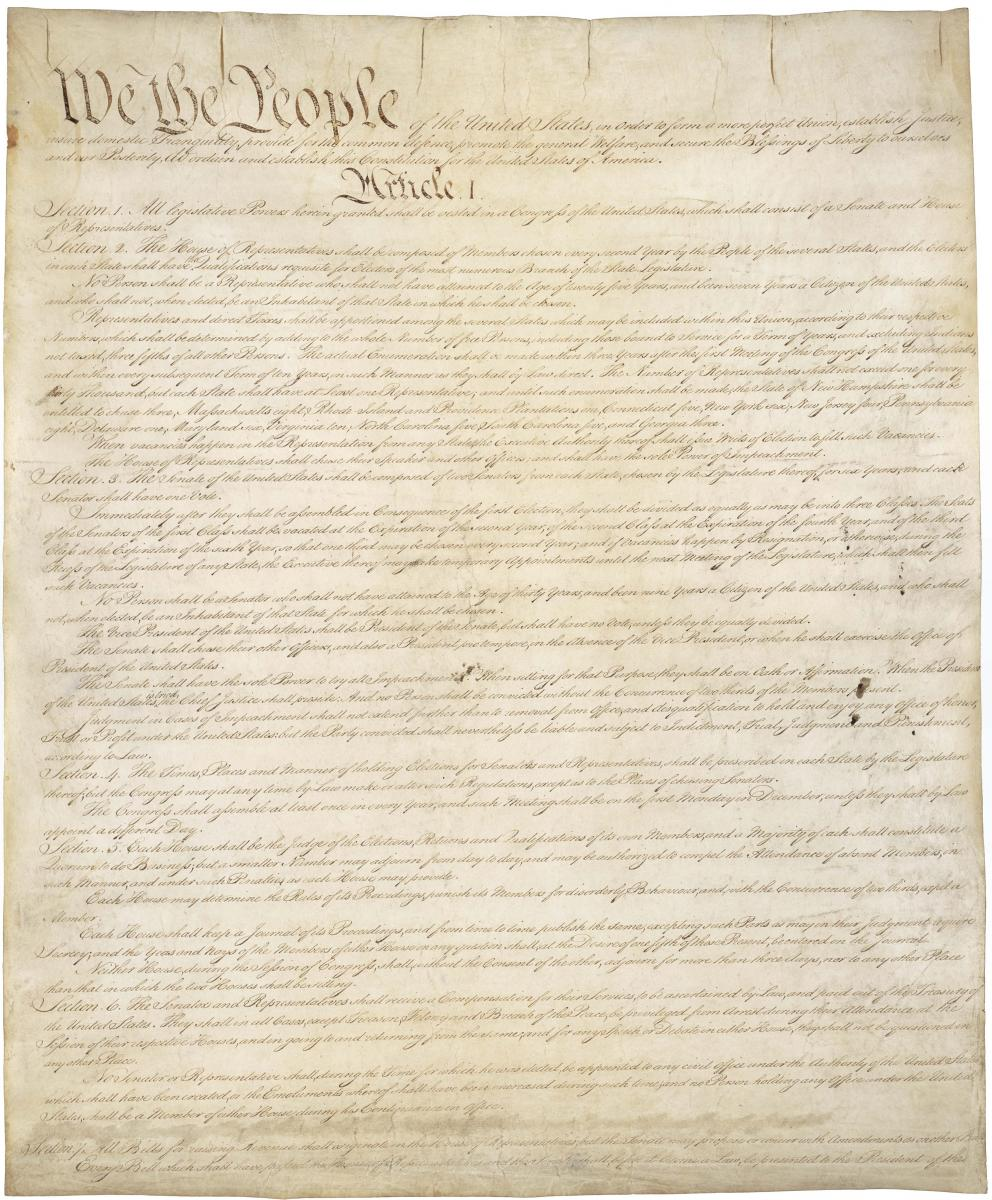
\includegraphics[scale=0.2]{zdroje/const.jpg}
\end{center}
\end{frame}

\begin{frame}{Bez určeného počtu}
%Q"9000/11000		O1"20000	O2"100000
\begin{itemize}
\item Předem zvolené $Q$
\item Počet hlasu pro stranu $H_{x}$
\item Zisk mandátů: $\left\lfloor\dfrac{H_{x}}{Q}\right\rfloor$
\end{itemize}
\end{frame}

\begin{frame}{Metoda nejvyšších zbytků}
\begin{itemize}
\item Počet rozdělovaných mandátů $N$
\item $Q=\dfrac{H_{c}}{N}$
\item Zisk mandátů: $\left\lfloor\dfrac{H_{x}}{Q}\right\rfloor+\{0;1\}$
\end{itemize}
\end{frame}

\begin{frame}{Paradox nových států}
\begin{center}
\begin{tabular}{|c|c|c|c|}
\hline 
100 k. & Obyvatelé & Ku kvótě & Křesla \\ 
\hline 
A & 8955 & \hspace{0.35cm}8955/100=89.55\hspace{0.35cm} & 90 \\ 
\hline 
B & 1045 & 1045/100=10.45 & 10 \\ 
\hline 
\end{tabular}
\end{center} 
\begin{center}
\begin{tabular}{|c|c|c|c|}
\hline 
105 k. & Obyvatelé & Ku kvótě & Křesla \\ 
\hline 
A & 8955 & 8955/100.14=89.42 & 89 \\ 
\hline 
B & 1045 & 1045/100.14=10.44 & 11 \\ 
\hline 
C & 515 & 515/100.14=5.14 & 5 \\ 
\hline 
\end{tabular} 
\end{center}
\end{frame}

\begin{frame}{Alabamský paradox}
\begin{center}
\begin{tabular}{|c|c|c|c|c|c|}
\hline 
 &  & \multicolumn{2}{c|}{10 křesel} & \multicolumn{2}{c|}{11 křesel} \\ 
\hline 
 & Obyvatelé & Poměr & Zisk & Poměr & Zisk \\ 
\hline 
A & 600 & 4,286 & 4 & 4,714 & 5 \\ 
\hline 
B & 600 & 4,286 & 4 & 4,714 & 5 \\ 
\hline 
C & 200 & 1,426 & 2 & 1.571 & 1 \\ 
\hline
\end{tabular} 
\end{center}
\end{frame}

\begin{frame}{Metoda nejvyšších průměrů}
\begin{itemize}
\item Počet rozdělovaných mandátů $N$
\item Zisk mandátů: $\left\{\dfrac{H_{x}}{Q}\right\}$
\item $\{$\hspace{0.25cm}$\{$
\item $Q$ je určeno tak, aby bylo rozděleno právě $N$ křesel.
\end{itemize}
\end{frame}

https://www.census.gov/population/apportionment/about/history.html

\end{document}
